\documentclass[11pt,answers]{exam}
\usepackage[legalpaper,bindingoffset=0in,left=.6in,right=0.8in,top=0.4in,bottom=0.7in,headsep=.5\baselineskip]{geometry}
\usepackage[utf8]{inputenc}
\usepackage{graphicx}
\usepackage{listings}
\usepackage{enumitem}
\usepackage{amsmath}
\usepackage{multirow}
\usepackage{multicol}
\usepackage{caption}
\usepackage{tabularx}
\usepackage{url}
\usepackage{amssymb}
\usepackage{array}
\usepackage{tikz}
\usepackage{graphicx}
\usetikzlibrary{shapes.callouts, patterns, positioning, arrows.meta, shapes.geometric, shadows, calc, patterns, 3d, backgrounds, shadings}
\usepackage{adjustbox}
\usepackage{ragged2e}
\usepackage{pgfplots}
\usepackage{fontawesome5}

%\pagenumbering{gobble}
\def\changemargin#1#2{\list{}{\rightmargin#2\leftmargin#1}
\item[]}
\let\endchangemargin=\endlist
\usepackage{xcolor}
\usepackage{listings}
\definecolor{mGreen}{rgb}{0,0.6,0}
\definecolor{mGray}{rgb}{0.5,0.5,0.5}
\definecolor{mPurple}{rgb}{0.58,0,0.82}
\definecolor{backgroundColour}{rgb}{0.95,0.95,0.92}
\lstset{
  language=C,
  basicstyle=\ttfamily\small,
  aboveskip={1.0\baselineskip},
  belowskip={1.0\baselineskip},
  columns=fixed,
  extendedchars=true,
  breaklines=true,
  tabsize=4,
  prebreak=\raisebox{0ex}[0ex][0ex]{\ensuremath{\hookleftarrow}},
  frame=lines,
  showtabs=false,
  showspaces=false,
  showstringspaces=false,
  keywordstyle=\color[rgb]{0.627,0.126,0.941},
  commentstyle=\color[rgb]{0.133,0.545,0.133},
  stringstyle=\color[rgb]{01,0,0},
  numbers=left,
  numberstyle=\small,
  stepnumber=1,
  numbersep=10pt,
  captionpos=t,
escapeinside={\%*}{*)}
}
%\renewcommand\thequestion{Q.\arabic{question}}
%\renewcommand{\questionlabel}{\thequestion)}
%\renewcommand{\questionshook}{%
%\setlength{\leftmargin}{0pt}%
%\setlength{\labelwidth}{-\labelsep}%
%}

%\pointsinrightmargin
\pointsdroppedatright
%\marksnotpoints
%\marginpointname{ \points}
%\pointformat{\boldmath\themarginpoints}

\title{
\begin{changemargin}{0.68cm}{0.68cm}
  \normalsize Makeup Class Test\hfill {January 2025}\\
\end{changemargin}
\vspace{.4cm}
\large BANGLADESH UNIVERSITY OF ENGINEERING AND TECHNOLOGY\\
\vspace{.1cm}
Department of Computer Science and Engineering\\
\vspace{.2cm}
L-4/T-1 \hspace{.1cm} CSE 409: Computer Graphics\\
\vspace{.2cm}
\textbf{Time: 25 minutes} \hspace{2.2cm} \textbf{Marks: 20}
\begin{changemargin}{0.68cm}{0.68cm}
  \normalsize Student Name: \underline{\hspace{6.5cm}} \hfill Student ID: \underline{\hspace{2.5cm}}\\
\end{changemargin}
}
\author{}
\date{}

\begin{document}

\maketitle
\thispagestyle{empty}
\begin{questions}
\vspace{-2cm}

\question[]{
a) What is the physical signification of attenuation of point light?
\hfill (2) \\

\vspace*{3cm}

b) Describe how textures can be used to enhance the Phong model.
\hfill (2) \\

\vspace*{3cm}

c) What is the advantage of using the Blinn-Phong model over the Phong model?
\hfill (2)

\vspace*{3cm}
}

\question[]
{
\begin{multicols}{2}
As a game developer in Iron studio, you are working in a new level of a game.
There is just a strange floor at $y=0$ and a spot light at $(1,10,0)$.\\
You have decided the following parameters using the Phong model for the floor:
\begin{itemize}
\item Spot light intensity $\mathbf{I} = (10, 10, 10)$
\item Falloff exponent $e = 5$
\item Ambient light $\mathbf{I}_a = (0.1, 0.1, 0.1)$
\item Ambient Coefficient $\mathbf{k}_a = (0.1, 0.2, 0.1)$
\item Diffuse Coefficient $\mathbf{k}_d = (0.8, 0.2, 0.6)$
\item Specular Coefficient $\mathbf{k}_s = (0.1, 0.6, 0.3)$
\item Shininess $n = 10$
\end{itemize}
The user begins as a flying soul at $(-4,3,0)$ and looks at the floor at $P(0,0,0)$.
\vfill
\columnbreak
\centering
\begin{tikzpicture}
\draw[black] (-6,-0.8) -- (1,-0.8);
\fill[pattern=north east lines, pattern color=gray] (-6,-0.8) rectangle (1,-1);
\draw[black,fill=black] (-2,-0.8) circle (1pt) node[above] {$P(0,0,0)$};

\draw[gray!70,very thin,->] (-5,1.8) --++(1,-1);
% stick man
\draw[fill=gray!30] (-5,1.8) circle (0.4cm);
\node at (-5,1.8) {\faIcon{eye}};

\node[above] at (-5,0.7) {$(-4,3,0)$};

\begin{scope}[shift={(-1,3.25)}]
  \draw[->] (0,0) -- (0,-1.5);
  \draw[-, gray!70] (0,0) -- (-120:1.5);
  \draw[-] (0, -0.75) arc [start angle=-90, end angle=-120, radius=0.75cm];
  \foreach \t in {0, 30, ..., 360} {
    \draw[very thin] (0,0) -- (\t:0.35);
  }
  \draw[black,fill=gray!30] (0,0) circle (3.5pt);
  \node[above] at (0,0.5) {$(1,10,0)$};
  \node at (-0.25, -1) {\scriptsize $30^\circ$};
\end{scope}

\end{tikzpicture}
\end{multicols}

a) What is the colour at $P$ using the Phong model?  \hfill (3)

\vspace*{2cm}
}
\newpage
b) What is the colour at $P$ using the Blinn-Phong model?  \hfill (3)
\vspace*{6cm}
\question[]
{
\begin{multicols}{2}

You are visiting the great pyramid of Giza. You are standing 300 meters west
at $(-300, 0, 0)$. The pyramid has its base between $(120, 0, 120)$, $(120, 0, -120)$, $(-120, 0, -120)$ and $(-120, 0, 120)$.
The top of the pyramid is at $(0, 200, 0)$.
It is 10 AM in the morning. The sun is pointing in the direction $-\hat{i} - 2\hat{j}$.

\vfill
\columnbreak
\begin{center}
\footnotesize
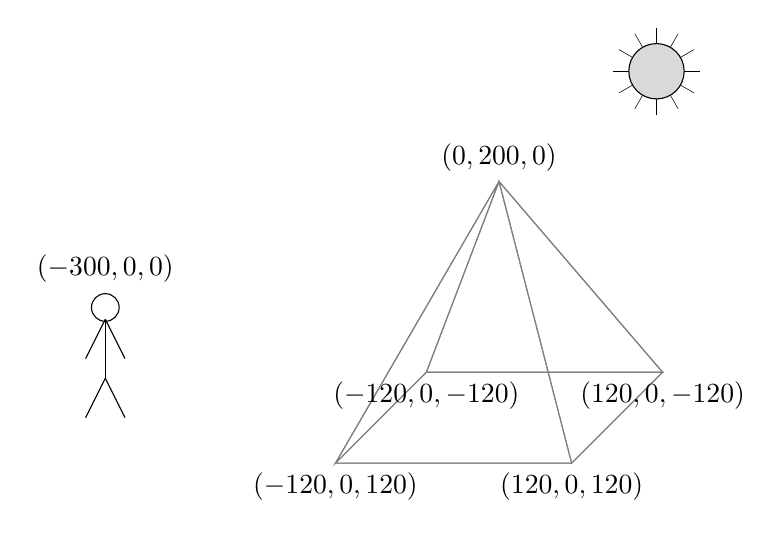
\begin{tikzpicture}

% stick man
\draw[black] (-5,0.35) --++(0,-0.75);
\draw[black] (-5,0.35) --++(-0.25,-0.5);
\draw[black] (-5,0.35) --++(0.25,-0.5);
\draw[black] (-5,-0.4) --++(-0.25,-0.5);
\draw[black] (-5,-0.4) --++(0.25,-0.5);
\draw[black] (-5,0.5) circle (5pt);

\node[above] at (-5,0.7) {$(-300,0,0)$};

\begin{scope}[shift={(2,3.5)}]
\foreach \t in {0, 30, ..., 360} {
  \draw[very thin] (0,0) -- (\t:0.55);
}
\draw[black,fill=gray!30] (0,0) circle (10pt);

\end{scope}
\begin{scope}[shift={(0,-0.9)},scale=1.5]
\draw[black!50] (1, 0, 1) -- (1, 0, -1) -- (-1, 0, -1) -- (-1, 0, 1) -- cycle;
\draw[black!50] (1, 0, 1) -- (1, 0, -1) -- (0,2,0) -- cycle;
\draw[black!50] (-1, 0, -1) -- (-1, 0, 1) -- (0,2,0) -- cycle;
\draw[black!50] (1, 0, 1) -- (-1, 0, 1) -- (0,2,0) -- cycle;
\draw[black!50] (1, 0, -1) -- (-1, 0, -1) -- (0,2,0) -- cycle;
\node[above] at (0, 2, 0) {$(0,200,0)$};
\node[below] at (1, 0, 1) {$(120,0,120)$};
\node[below] at (1, 0, -1) {$(120,0,-120)$};
\node[below] at (-1, 0, -1) {$(-120,0,-120)$};
\node[below] at (-1, 0, 1) {$(-120,0,120)$};
\end{scope}

\end{tikzpicture}

\end{center}
\end{multicols}

Are you in the shadow of the pyramid? \hfill (6)
\vspace{0.5cm}

Hint 1: Consider a shadow ray.

Hint 2: Does the shadow ray intersect the pyramid at all?
}
\vspace{14cm}
\question[]For your hard work and attending the exam.\hfill (2)

\end{questions}
\end{document}